\documentclass{oblivoir}
\usepackage{amsmath,amssymb,amsthm,kotex,paralist,kswrapfig}

\usepackage[skipabove=10pt]{mdframed}

\usepackage{tabto,pifont}
\TabPositions{0.2\textwidth,0.4\textwidth,0.6\textwidth,0.8\textwidth}
\newcommand\tabb[5]{\par\bigskip\noindent
\ding{172}\:{\ensuremath{#1}}
\tab\ding{173}\:\:{\ensuremath{#2}}
\tab\ding{174}\:\:{\ensuremath{#3}}
\tab\ding{175}\:\:{\ensuremath{#4}}
\tab\ding{176}\:\:{\ensuremath{#5}}}

\usepackage{enumitem}
%\setlist{noitemsep}
\setlist[enumerate]{label=(\arabic*)}

\newcounter{num}
\newcommand{\prob}[1]
{\bigskip\noindent\refstepcounter{num}\textbf{문제 \arabic{num}) #1}\par\noindent}

\newcommand{\ans}{
{\par
\raggedleft\textbf{답 : (\qquad\qquad\qquad\qquad\qquad\qquad)}
\par}\bigskip\bigskip}

\newcommand\ov[2]{\ensuremath{\overline{#1#2}}}
\newcommand\wh[2]{\ensuremath{\widehat{#1#2}}}
\newcommand{\pa}{\mathbin{\:\!/\mkern-5mu/\!\:}}

%\newcommand{\pb}[1]%\Phantom + fBox
%{\fbox{\phantom{\ensuremath{#1}}}}

%%%%
\begin{document}

\title{윤영 : 05 쎈(3)}
\author{}
\date{\today}
\maketitle

\setcounter{section}{20}
%%
\section{원주각}


\prob{994}
\kswrapfig[Pos=r,Width=5cm]{994}{
오른쪽 그림과 같이 두 원 \(O\)와 \(O'\)이 내접하고 있고, 원 \(O\)의 반지름의 길이는 원 \(O'\)의 지름의 길이와 같다.
\ov AP는 원 \(O'\)의 접선이고 \ov AB=18cm일 때, \ov AQ의 길이를 구하여라.
}
\tabb{6\text{cm}}{6\sqrt2\text{cm}}{12\text{cm}}{12\sqrt2\text{cm}}{12\sqrt3\text{cm}}

%
\prob{1028a}
\kswrapfig[Pos=r,Width=5cm]{1028a}{
오른쪽 그림에서 \(\square ABCD\)는 원에 내접하고 \wh AE=\wh DE이다.
\(\angle BCE=72^\circ\)일 때, \(\angle x\)의 크기를 구하여라.
}
\tabb{99^\circ}{108^\circ}{117^\circ}{126^\circ}{135^\circ}

\clearpage
%
\prob{1028b}
\kswrapfig[Pos=r,Width=5cm]{1028b}{
오른쪽 그림과 같이 \(\angle BAC=75^\circ\)인 \(\triangle ABC\)의 내접원 위에 \wh AD=\wh CE가 되도록 \(D\)와 \(E\)를 잡았다.
\ov AE와 \ov BD의 교점을 \(P\)라고 할 때, \(\angle DPE\)의 크기를 구하시오.
}
\tabb{100^\circ}{105^\circ}{110^\circ}{115^\circ}{120^\circ}

%
\prob{1039}
\kswrapfig[Pos=r,Width=5cm]{1039}{
오른쪽 그림에서 \(\square ABCD\)는 원 \(O\)에 내접하고 \(\angle DPC=35^\circ\), \(\angle BQC=55^\circ\)일 때, \(\angle BAD\)의 크기는?
}
\tabb{108^\circ}{120^\circ}{126^\circ}{135^\circ}{144^\circ}

%
\prob{1049}
\kswrapfig[Pos=r,Width=5cm]{1049}{
오른쪽 그림과 같이 반지름의 길이가 모두 \(2\)인 세 원 \(O\), \(O'\), \(O''\)이 서로 다른 원의 중심을 지날 때, \wh A{O'}+\wh C{O'}의 값을 구하여라.
}
\tabb{\frac23\pi}{\frac56\pi}{\pi}{\frac76\pi}{\frac43\pi}

%
\prob{1053a}
\kswrapfig[Pos=r,Width=5cm]{1053a}{
오른쪽 그림의 원 \(O\)에서 \wh AB=\wh CD이고 \(\angle APB=55^\circ\)일 때, \(\angle EOC\)의 크기를 구하여라.
}
\tabb{110^\circ}{115^\circ}{120^\circ}{125^\circ}{130^\circ}

%
\prob{1053b}
\kswrapfig[Pos=r,Width=5cm]{1053b}{
오른쪽 그림의 원 \(O\)에서 \wh AB=\wh CE이고 \(\angle APB=60^\circ\)일 때, \(\angle COD\)의 크기를 구하여라.
}
\tabb{110^\circ}{115^\circ}{120^\circ}{125^\circ}{130^\circ}

%
\prob{1055a}
\kswrapfig[Pos=r,Width=5cm]{1055a}{
오른쪽 그림의 원 \(O\)에서 두 현 \(AB\)와 \(CD\)의 교점 \(P\)에 대하여 \(\angle APD=105^\circ\)이다.
\(\wh AD=2\pi\), \(\wh BC=5\pi\)일 때, 원 \(O\)의 반지름의 길이를 구하여라.
}
\tabb56789

\clearpage
%
\prob{1055b}
\kswrapfig[Pos=r,Width=5cm]{1055b}{
오른쪽 그림과 같이 \ov AB를 지름으로 하는 원 \(O\)에 대하여 \(\angle ABC=40^\circ\)이고 \(\wh BC=5\pi\)일 때, 원 \(O\)의 반지름의 길이를 구하여라.
}
\tabb56789

%
\prob{1061}
\kswrapfig[Pos=r,Width=5cm]{1061}{
오른쪽 그림에서 \(\ov AD\pa\ov CF\)이고 \(\angle ADB=17^\circ\), \(\angle BFC=32^\circ\)일 때, \(\angle x+\angle y\)의 값을 구하여라.
}
\tabb{90^\circ}{92^\circ}{94^\circ}{96^\circ}{98^\circ}

%%
\section{원주각의 활용}

%
\prob{1109a}\label{orthocenter}
\kswrapfig[Pos=r,Width=5cm]{1109a}{
오른쪽 그림에서 \(H\)는 \(\triangle ABC\)의 세 꼭짓점에서 대변에 내린 수선의 교점이다.
다음 사각형 중 원에 내접하지 않는것은?
}
\par\bigskip\noindent
\ding{172}\:{\(\square AFHE\)}
\tab\tab\ding{173}\:\:{\(\square ABDE\)}
\tab\tab\ding{174}\:\:{\(\square BDHF\)}
\tab\ding{175}\:\:{\(\square CAFD\)}
\tab\tab\ding{176}\:\:{\(\square AFDE\)}

%
\prob{1109b}
\kswrapfig[Pos=r,Width=5cm]{1109b}{
오른쪽 그림에서 \(H\)는 \(\triangle ABC\)의 세 꼭짓점에서 대변이나 대변의 연장선에 내린 수선의 교점이다.
한 원 위에 있지 않은 네 점은?
}
\par\bigskip\noindent
\ding{172}\:{\(A\), \(F\), \(E\), \(H\)}
\tab\tab\ding{173}\:\:{\(A\), \(B\), \(E\), \(D\)}
\tab\tab\ding{174}\:\:{\(B\), \(H\), \(D\), \(F\)}
\tab\ding{175}\:\:{\(C\), \(D\), \(A\), \(F\)}
\tab\tab\ding{176}\:\:{\(A\), \(F\), \(E\), \(D\)}
%\tabb{A,\:F,\:H,\:E}{A,\:B,\:D,\:E}{B,\:D,\:H,\:F}{C,\:A,\:F,\:D}{A,\:F,\:D,\:E}

\bigskip\bigskip
\kswrapfig[Pos=r,Width=5cm]{1109c}{
문제 \ref{orthocenter}에서 \ov AH=4, \ov BD=15, \ov CD=3이라고 하자.
\(B\), \(D\), \(H\), \(F\)가 한 원 위에 있음을 이용하여 다음 물음에 답하여라.
(문제 13--16)
}

%
\prob{1109c}
\(\triangle CDH\)와 닮음인 삼각형을 고르시오.
\tabb{\triangle HEC}{\triangle CDA}{\triangle ADB}{\triangle HFB}{\triangle ABC}

%
\prob{1109d}
\ov DH의 길이를 구하여라.
\tabb{\frac92}{5}{\frac{11}2}{6}{\frac{13}2}

%
\prob{1109e}
\ov AB, \ov AF의 길이를 차례로 구하여라.
\tabb
{3\sqrt{34},\:\frac4{17}\sqrt{34}}{3\sqrt{34},\:\frac5{17}\sqrt{34}}
{3\sqrt{34},\:\frac6{17}\sqrt{34}}{4\sqrt{34},\:\frac4{17}\sqrt{34}}
{4\sqrt{34},\:\frac5{17}\sqrt{34}}

\clearpage
%
\prob{1109f}
\(A\), \(F\), \(D\), \(C\)가 한 원 위에 있음을 이용하여, \ov CH와 \ov FH의 길이를 차례로 구하여라.
\tabb
{\sqrt{34},\:\frac5{17}\sqrt{34}\:}{\sqrt{34},\:\frac{10}{17}\sqrt{34}\:}
{\sqrt{34},\:\frac{15}{17}\sqrt{34}}{3\sqrt{34},\:\frac5{17}\sqrt{34}}
{3\sqrt{34},\:\frac{10}{17}\sqrt{34}}

% 1137의 3번을 변형한 그림, 1137의 5번그림 1158의 두 그림, 1183의 한 그림, 
\prob{1137, 1158, 1183}
다음 중 \(A\), \(B\), \(C\), \(D\)가 한 원 위에 있지 않은 것은?
\par\bigskip\noindent
\begin{tabular}{cc}
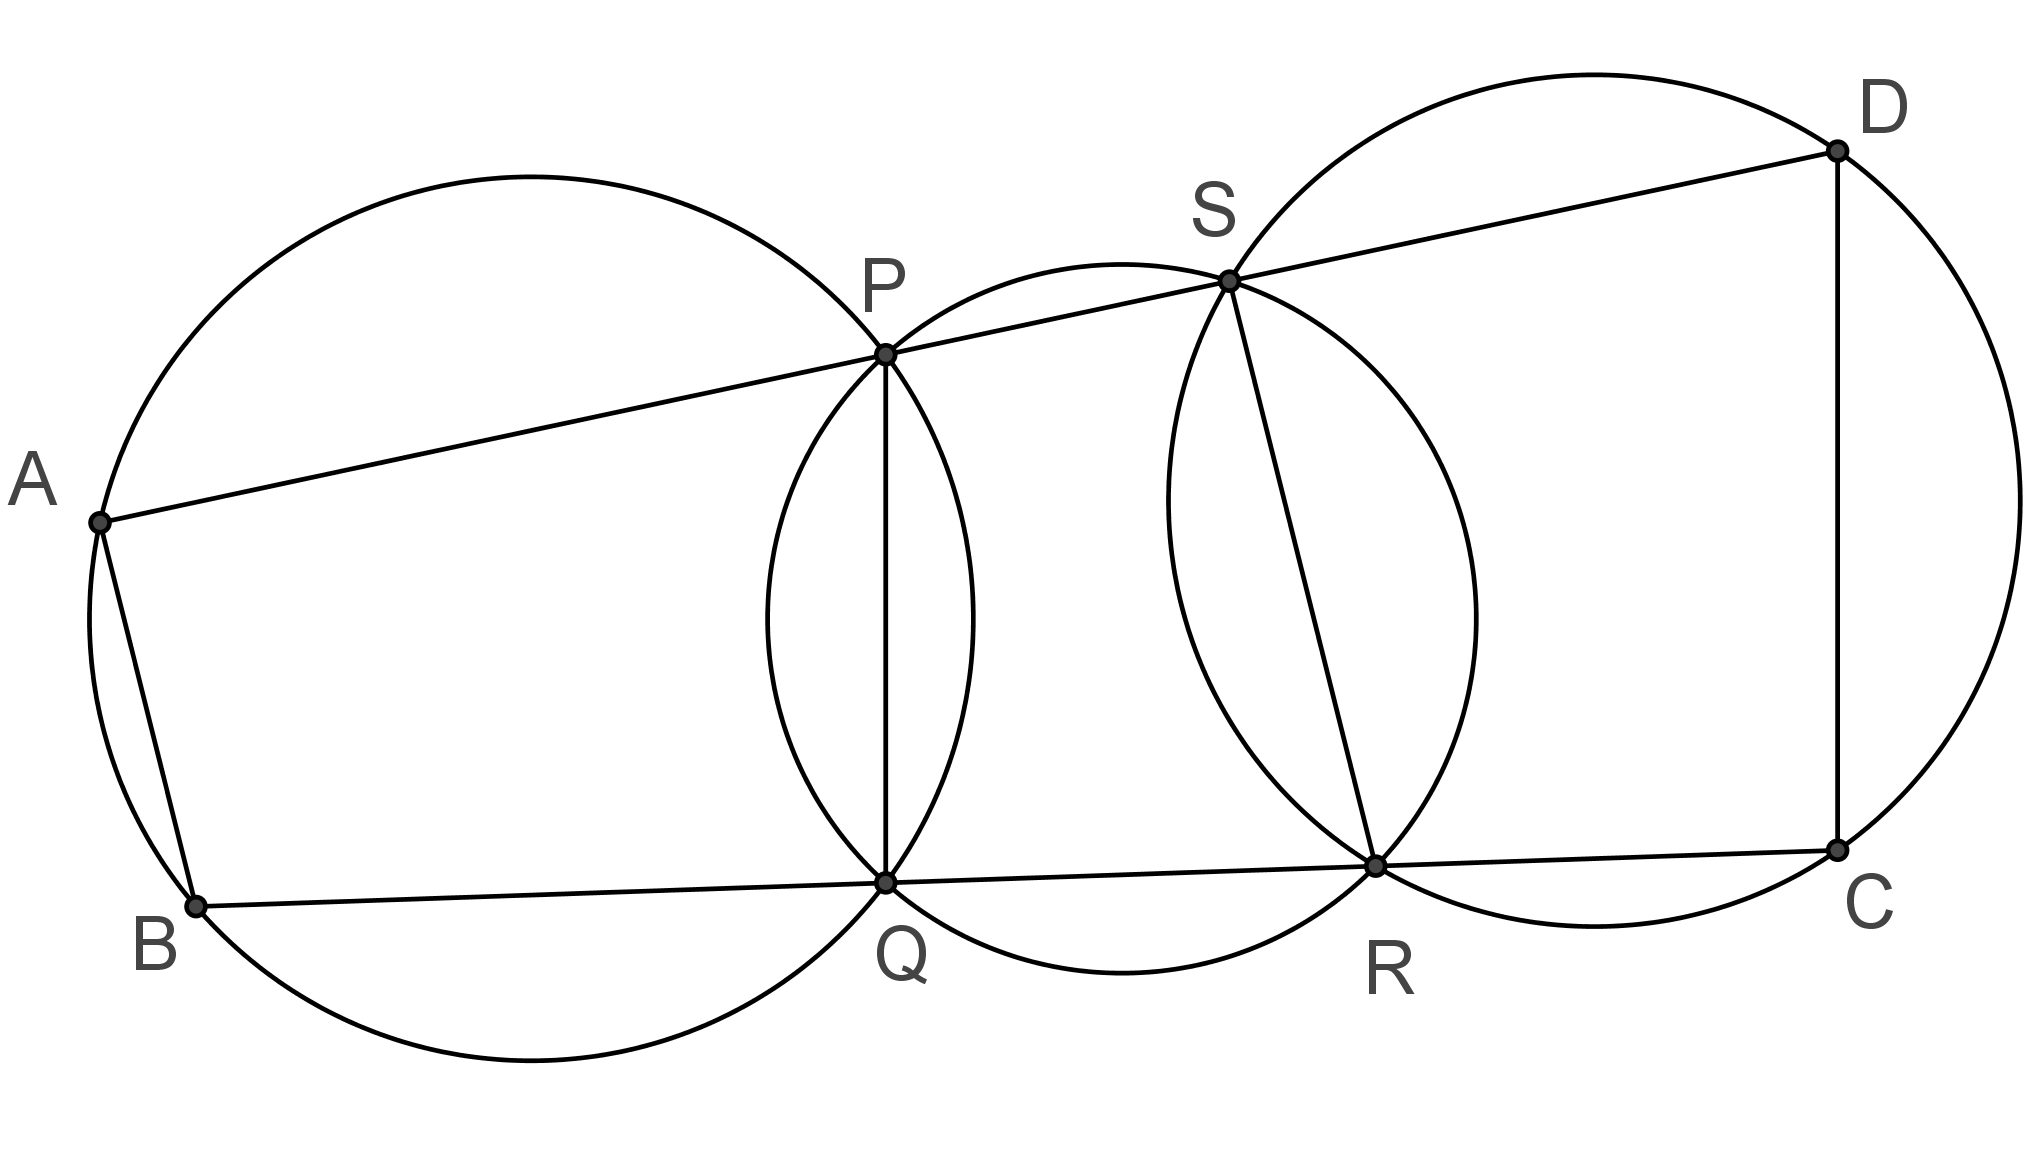
\includegraphics[width=0.4\textwidth]{1137a}&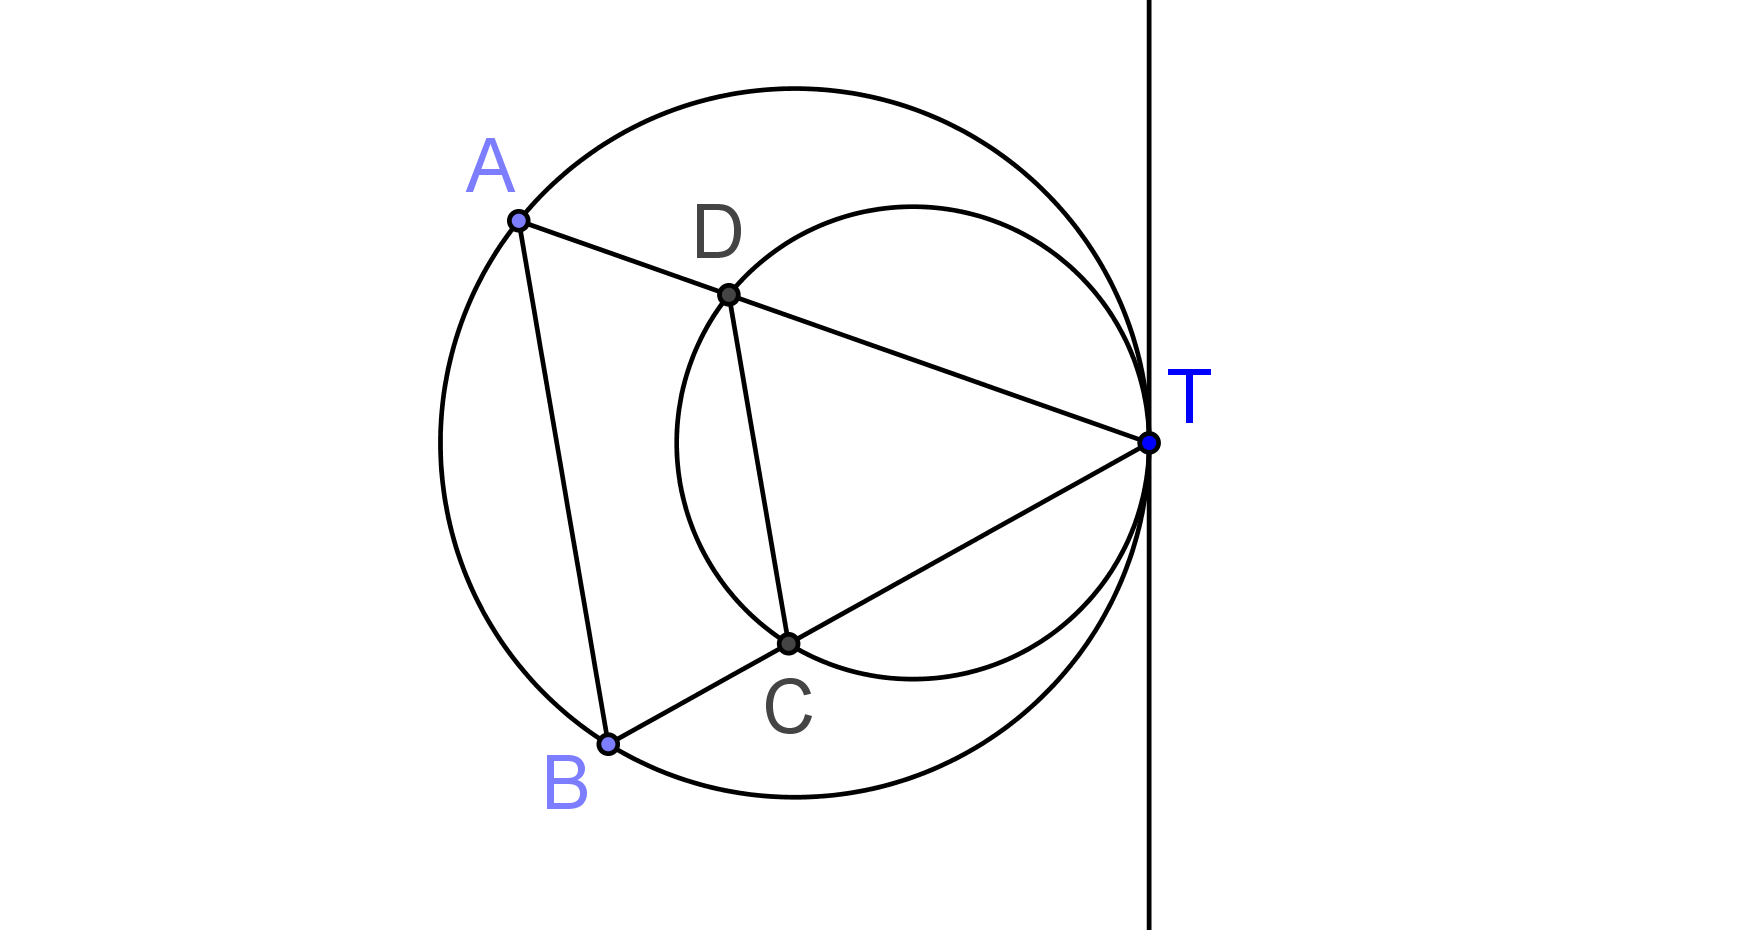
\includegraphics[width=0.4\textwidth]{1137b}\\
\ding{172}&\ding{173}\\
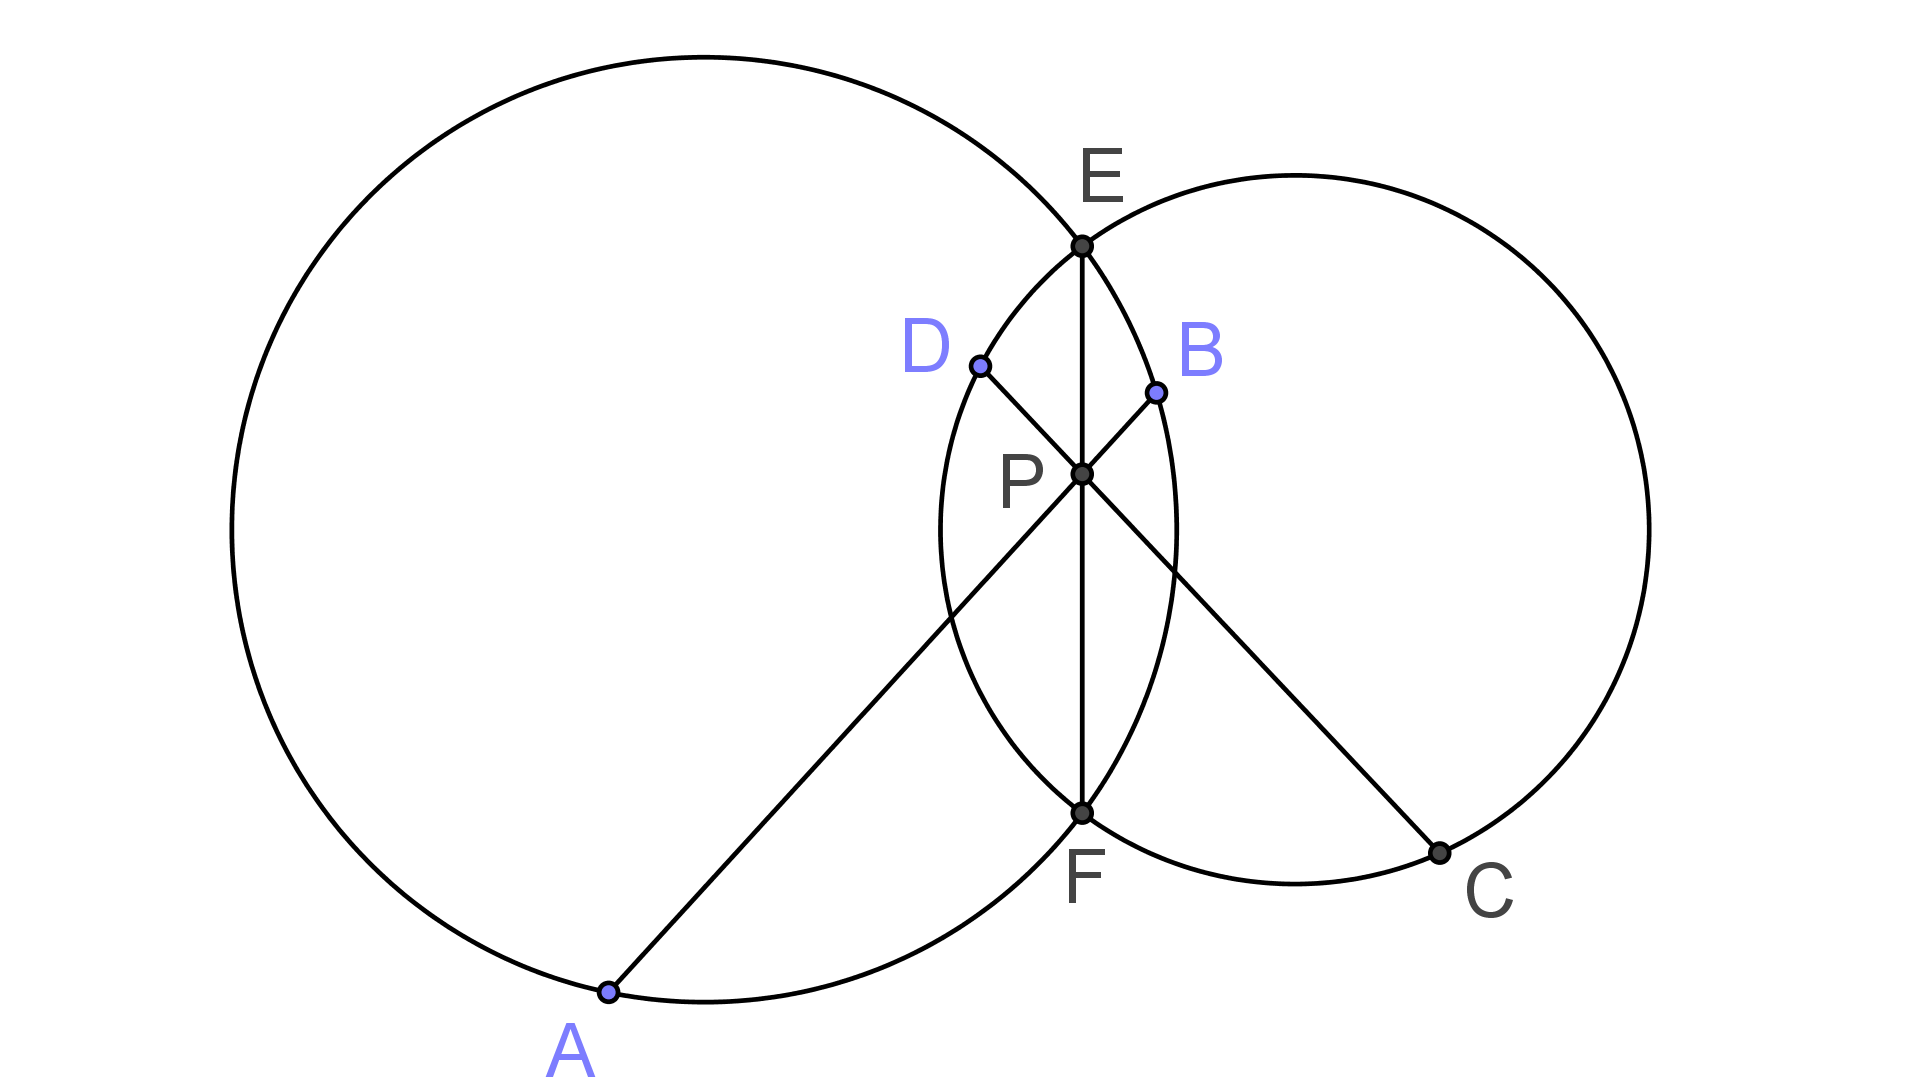
\includegraphics[width=0.4\textwidth]{1158a}&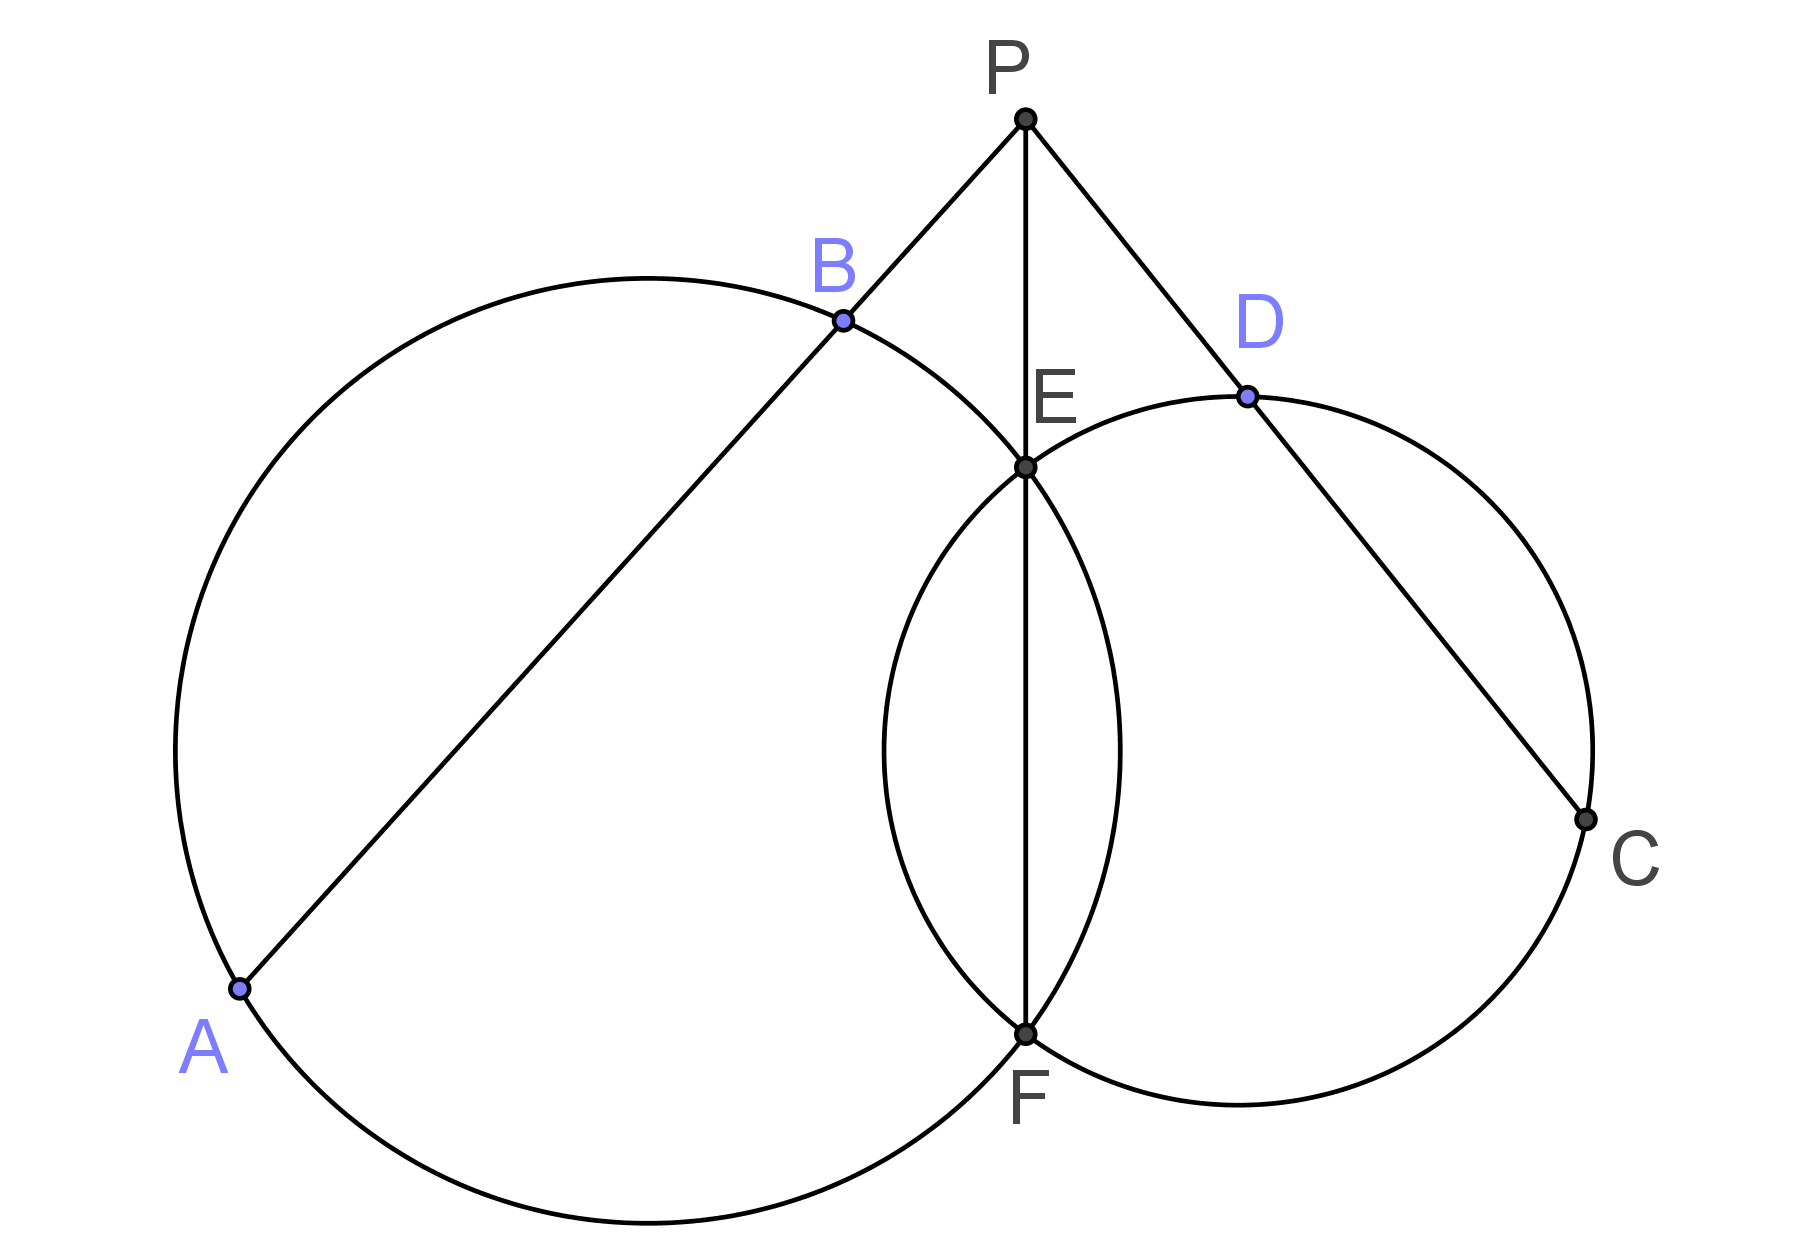
\includegraphics[width=0.4\textwidth]{1158b}\\
\ding{174}&\ding{175}\\
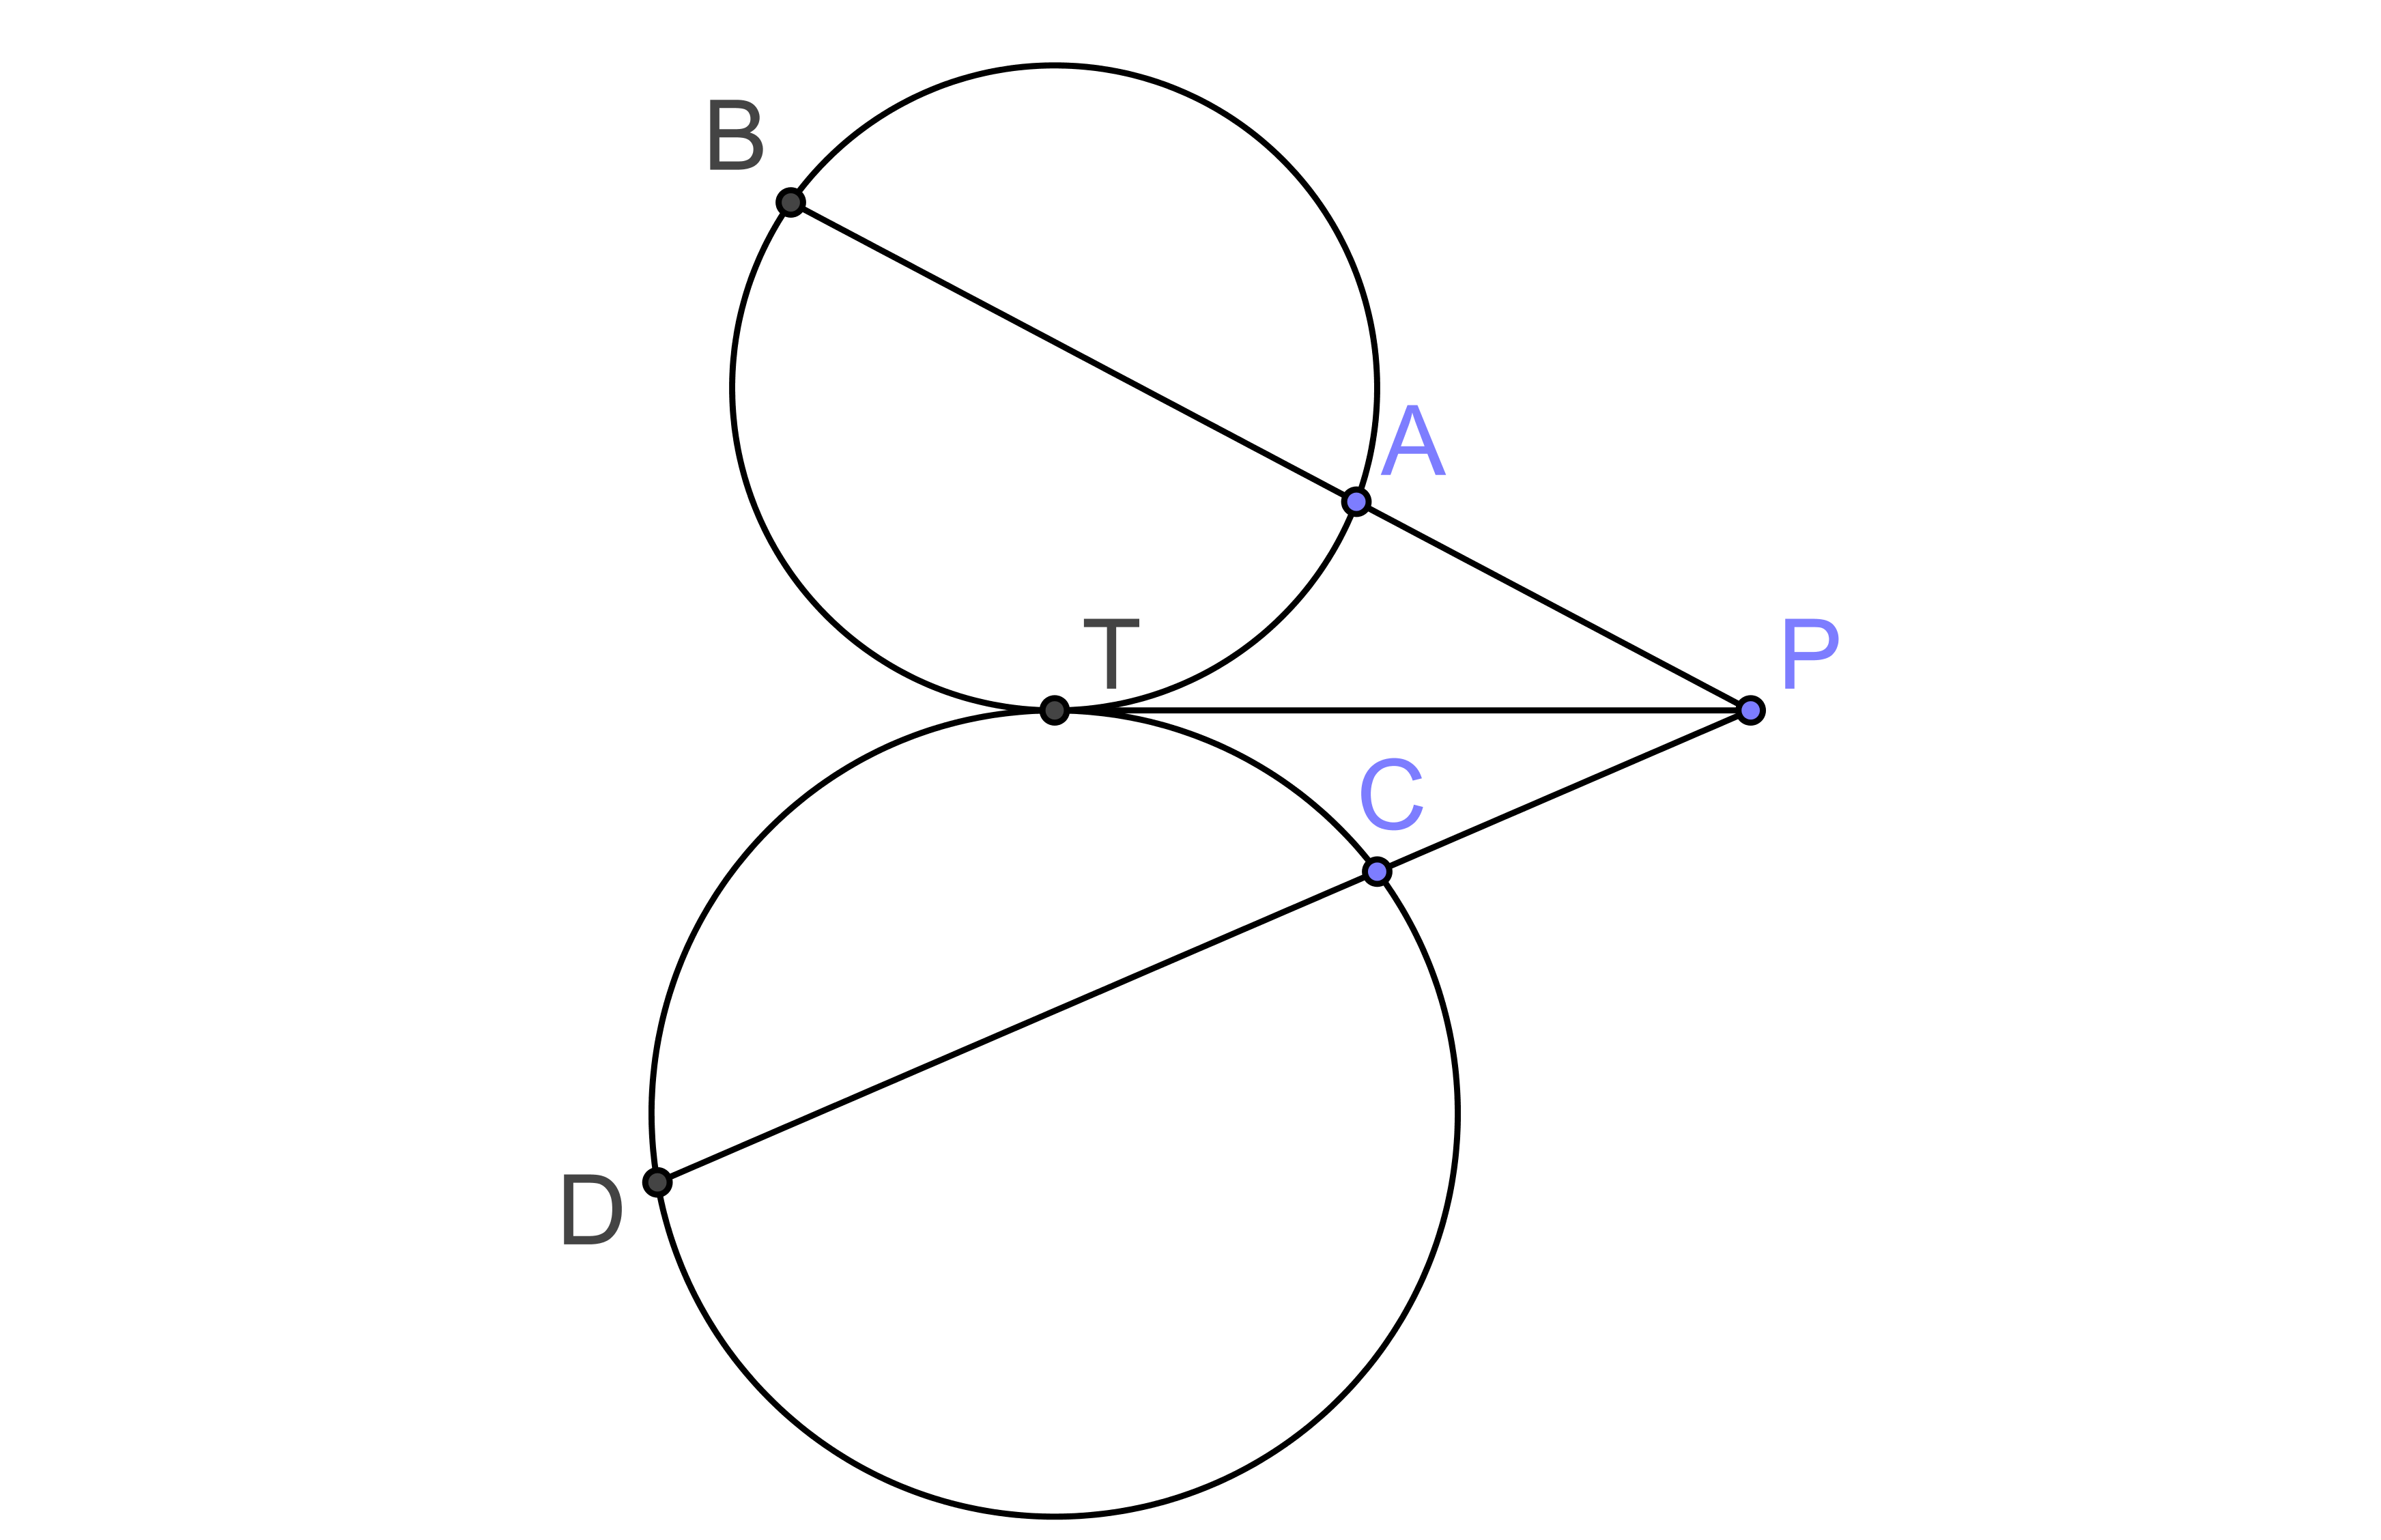
\includegraphics[width=0.4\textwidth]{1183}&\\
\ding{176}&\\
%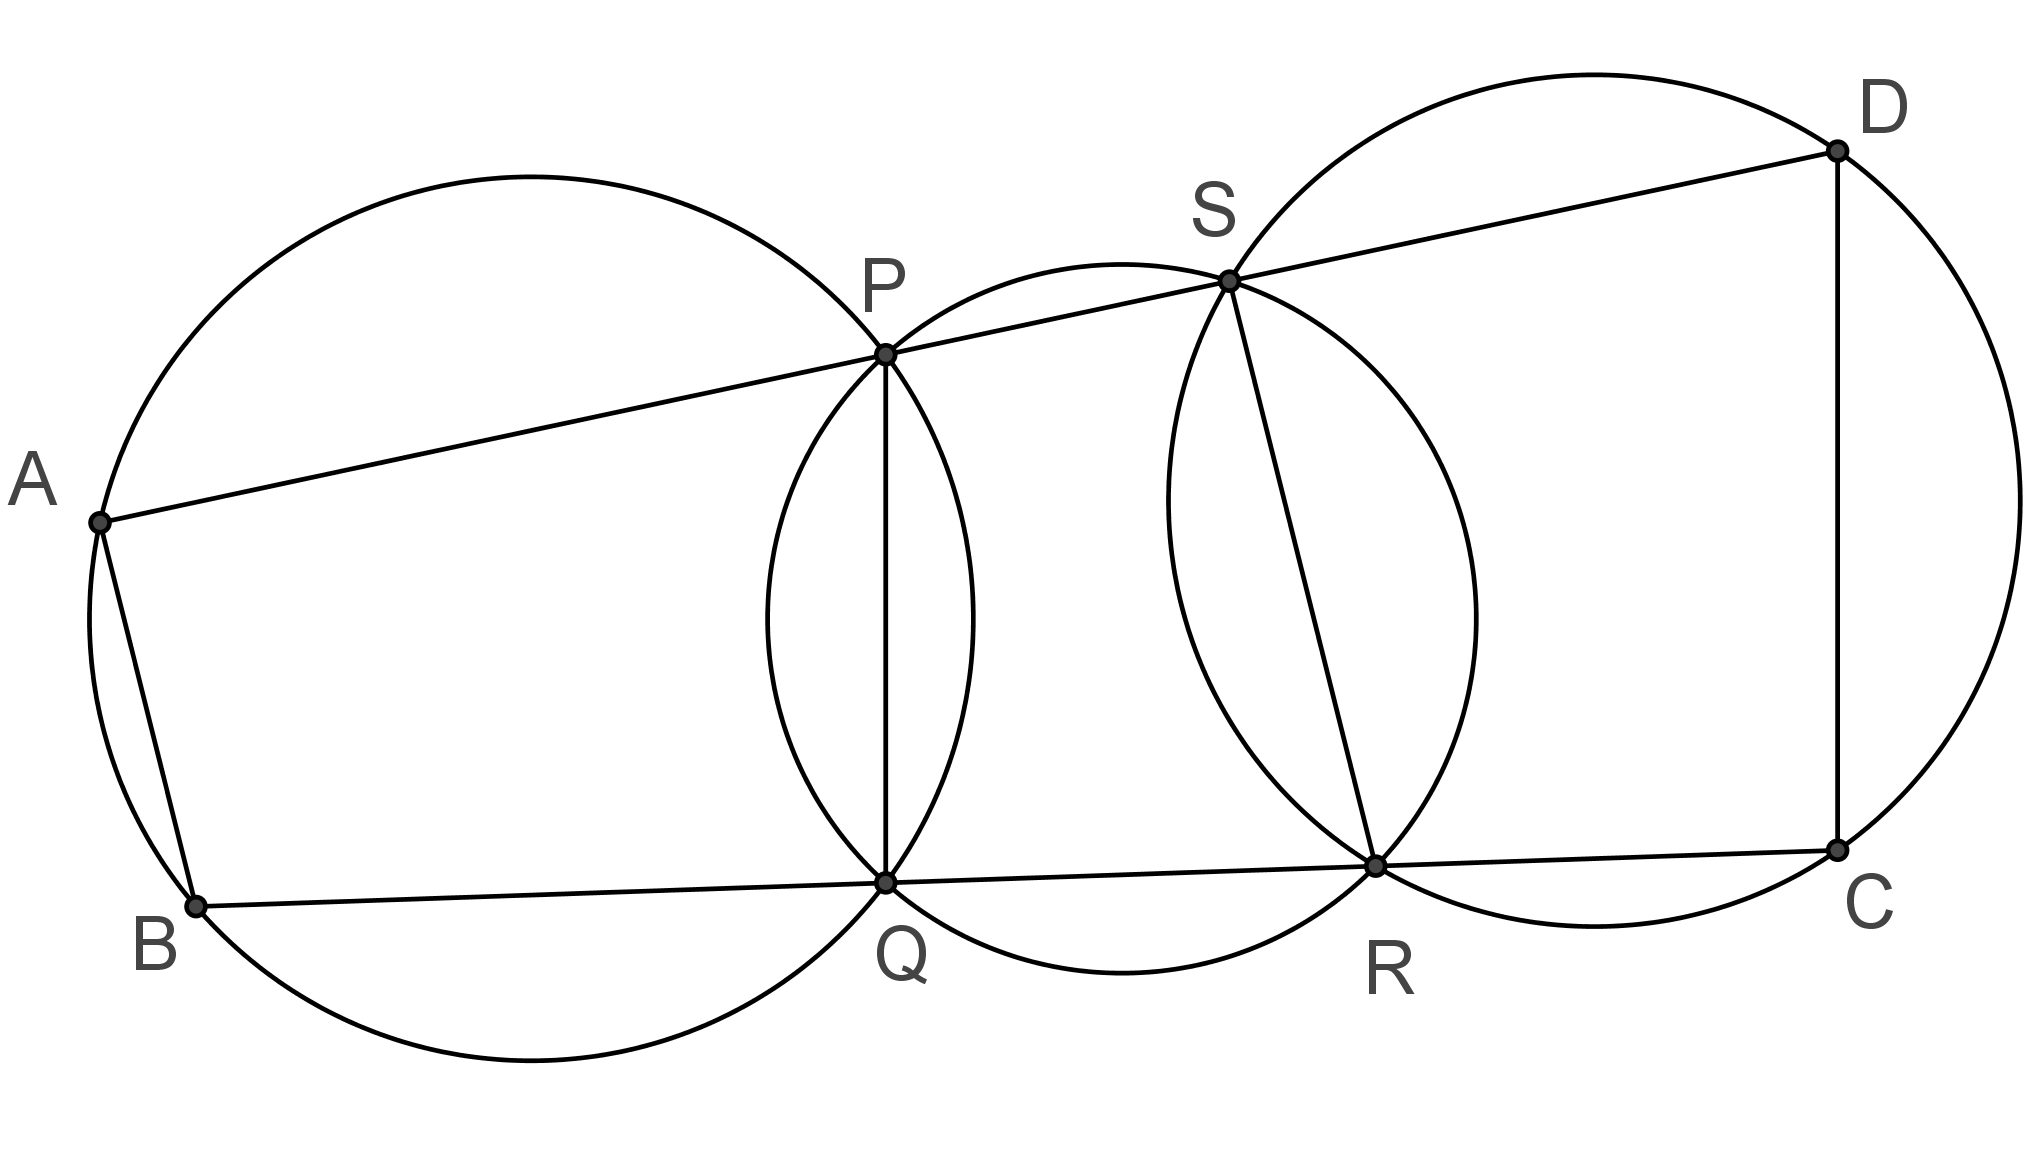
\includegraphics[width=0.4\textwidth]{1137a}
\end{tabular}

\clearpage
%
\prob{1172}
\kswrapfig[Pos=r,Width=5cm]{1172a}{
오른쪽 그림에서 \ov PT는 원 \(O\)의 접선이고 \(\angle BAT=30^\circ\), \ov AB=4cm일 때, \(\ov PT\)의 길이는?
}
\tabb{2\sqrt2\text{cm}}{2\sqrt3\text{cm}}{3\sqrt2\text{cm}}{3\sqrt3\text{cm}}{3\sqrt5\text{cm}}

%
\prob{1176}
\kswrapfig[Pos=r,Width=5cm]{1176}{
오른쪽 그림에서 \ov PT는 원 \(O\)의 접선이고 \ov AB=12, \ov AP=4, \ov AT=7일 때, \ov BT의 길이는?
}
\tabb{11}{12}{13}{14}{15}

%
\prob{1184(각이등분선)a}
\kswrapfig[Pos=r,Width=5cm]{1184a}{
오른쪽 그림에서 \ov AE는 \(\angle A\)의 이등분선이다.
\ov AB=15cm, \ov AC=4cm, \ov DE=4cm일 때, \ov AD의 길이를 구하여라.
}
\tabb{5\text{cm}}{6\text{cm}}{7\text{cm}}{8\text{cm}}{9\text{cm}}

\clearpage
%
\prob{1184(각이등분선)b}
\kswrapfig[Pos=r,Width=5cm]{1184b}{
오른쪽 그림에서 \ov AE는 \(\angle A\)의 이등분선이다.
\ov BD=3cm, \ov CD=4cm, \ov DE=2cm, \ov CE=4일 때, \ov AC의 길이를 구하여라.
}
\tabb{5\text{cm}}{6\text{cm}}{7\text{cm}}{8\text{cm}}{9\text{cm}}

%
\prob{1184(각이등분선)c}
\kswrapfig[Pos=r,Width=5cm]{1184c}{
오른쪽 그림에서 \ov AE는 \(\angle A\)의 이등분선이다.
\ov AD=9cm, \ov DE=3cm일 때, \ov BE+\ov CE의 값을 구하여라.
}
\tabb{8\text{cm}}{9\text{cm}}{10\text{cm}}{11\text{cm}}{12\text{cm}}

%
\prob{(이등변삼각형)a}
\kswrapfig[Pos=r,Width=5cm]{isosceles_a}{
오른쪽 그림에서 \ov AB=\ov AC이고, \(Q\)는 \wh BC 위의 점이다.
\ov AP=6cm, \ov PQ=2cm일 때, \ov AC의 길이를 구하여라.
}
\tabb{4\sqrt2\text{cm}}{4\sqrt3\text{cm}}{4\sqrt5\text{cm}}{4\sqrt6\text{cm}}{4\sqrt7\text{cm}}

\clearpage
%
\prob{(이등변삼각형)b}
\kswrapfig[Pos=r,Width=5cm]{isosceles_b}{
오른쪽 그림에서 \ov AB=\ov AC이고, \(Q\)는 \wh BC 위의 점이다.
\ov AC=6cm, \ov PQ=5cm일 때, \ov AQ의 길이를 구하여라.
}
\tabb{5\text{cm}}{6\text{cm}}{7\text{cm}}{8\text{cm}}{9\text{cm}}

%
\prob{1186(직각삼각형)}
\kswrapfig[Pos=r,Width=5cm]{1186a}{
오른쪽 그림에서 \ov AD가 원의 지름이고, \(\ov AH\perp\ov BC\)이다.
\ov AB=8cm, \ov AC=5cm, \ov AH=4cm일 때, 원 \(O\)의 반지름의 길이를 구하여라.
\tabb{5\text{cm}}{6\text{cm}}{7\text{cm}}{8\text{cm}}{9\text{cm}}
}
%
%%
%\prob{1186(직각삼각형)b}
%오른쪽 그림에서 \ov AD가 원의 지름이고, \(\ov AH\perp\ov BC\)이다.
%\ov AO=5cm, \ov BD=6cm, \ov CH=3cm일 때, \ov AH의 길이를 구하여라.

%
\prob{1187}
\kswrapfig[Pos=r,Width=5cm]{1187}{
오른쪽 그림과 같이 \ov AB를 지름으로 하는 반원 \(O\)에서 \(\angle OCP=\angle ODP=15^\circ\), \(\angle AOC=39^\circ\)일 때, \(\angle AOC\)의 크기는?
}
\tabb{5^\circ}{6^\circ}{7^\circ}{8^\circ}{9^\circ}

\clearpage
%
\prob{1189}
\kswrapfig[Pos=r,Width=5cm]{1189}{
오른쪽 그림과 같이 \(\triangle ABC\)의 외접원 \(O\)에서 현 \(BC\)의 연장선과 점 \(A\)에서 원에 그은 접선이 만나는 점을 \(D\)라고 하고, \(\angle ADB\)의 이등분선이 변 \(AB\)와 만나는 점을 \(E\)라고 하자.
\(\angle BAC=40^\circ\)일 때, \(\angle AED\)의 크기를 구하여라.
}
\tabb{50^\circ}{55^\circ}{60^\circ}{65^\circ}{70^\circ}

%
\prob{1190}
\kswrapfig[Pos=r,Width=5cm]{1190}{
오른쪽 그림과 같이 직선 \(PB\)는 원 \(O\)의 접선이고 \(\angle ABP=50^\circ\), \(\wh AB=10\pi\)cm이다.
이때 원 \(O\)의 반지름의 길이를 구하여라.
}
\tabb{9\text{cm}}{12\text{cm}}{15\text{cm}}{18\text{cm}}{21\text{cm}}

%%
%\prob{1193}
%오른쪽 그림에서 \ov AC, \ov BC는 각각 원 \(O\), \(O'\)의 지름이고 직선 \(AD\)는 원 \(O'\)의 접선일 때, \(\angle EBC\)의 크기를 구하여라.

%
\prob{1195}
\kswrapfig[Pos=r,Width=5cm]{1195}{
오른쪽 그림에서 직선 \(AB\)는 두 원 \(O\), \(O'\)의 공통인 접선이고 두 점 \(P\), \(Q\)는 두 원의 교점이다.
\(\angle PAQ=32^\circ\), \(\angle PBQ=24^\circ\)일 때, \(\angle APB\)의 크기를 구하여라.
}
\tabb{61^\circ}{62^\circ}{63^\circ}{64^\circ}{65^\circ}

\clearpage
%
\prob{1197}
\kswrapfig[Pos=r,Width=5cm]{1197}{
오른쪽 그림과 같이 원 \(O'\)이 원 \(O\)에 내접하고 \ov AC=8, \ov DE=6일 때, 원 \(O\)의 반지름의 길이를 구하여라.
}
\tabb{8.5\text{cm}}{9\text{cm}}{9.5\text{cm}}{10\text{cm}}{10.5\text{cm}}

%
\prob{1199}
\kswrapfig[Pos=r,Width=5cm]{1199}{
오른쪽 그림에서 \ov CD는 원 \(O\)의 지름이고 \ov AB는 접선이다 \ov AD=2cm, \ov BC=8cm일 때, \(\square ABCD\)의 넓이는?
}
\tabb{24\text{cm}^2}{28\text{cm}^2}{32\text{cm}^2}{36\text{cm}^2}{40\text{cm}^2}

%
\prob{1201}
\kswrapfig[Pos=r,Width=5cm]{1201}{
오른쪽 그림에서 \ov AB는 두 원 \(O\), \(O'\)의 공통인 현이고 \ov T{T'}는 공통인 접선이다.
\ov T{T'}=6cm, \ov AB=4cm, \(\triangle APT'=4\text{cm}^2\)일 때, \(\triangle BTT'\)의 넓이를 구하여라.
}
\tabb{64\text{cm}^2}{68\text{cm}^2}{72\text{cm}^2}{76\text{cm}^2}{80\text{cm}^2}

\clearpage
%
\prob{1204}
\kswrapfig[Pos=r,Width=5cm]{1204}{
오른쪽 그림에서 직선 \(TT'\)는 점 \(A\)에서 두 원과 접하고, 현 \(BC\)는 점 \(D\)에서 작은 원에 접한다.
\(\angle CBA=25^\circ\), \(\angle BAT'=65^\circ\)일 때, \(\angle y-\angle x\)의 크기를 구하여라.
}
\tabb{15^\circ}{20^\circ}{25^\circ}{30^\circ}{35^\circ}

%
\prob{1207}
\kswrapfig[Pos=r,Width=5cm]{1207}{
오른쪽 그림에서 직선 \(PT\)는 지름이 \ov AB인 원 \(O\)의 접선이고 점 \(C\)는 접점이다.
\(\ov AP\perp \ov PT\)이고 \ov AP=10cm, \ov AB=15cm일 때, \(\cos x\)의 값을 구하여라.
}
\tabb{\frac{\sqrt2}3}{\frac{\sqrt3}3}{\frac{\sqrt5}3}{\frac{\sqrt6}3}{\frac{\sqrt7}3}

\bigskip\bigskip
아래 그림에서 \(\ov AB\)는 반원 \(O\)의 지름이고 \ov AQ=9, \ov BQ=1, \(\ov AB\perp\ov PQ\)이다.
이때 다음 물음에 답하여라.
(문제 \ref{start}--\ref{end})

\begin{figure}[h!]
\centering
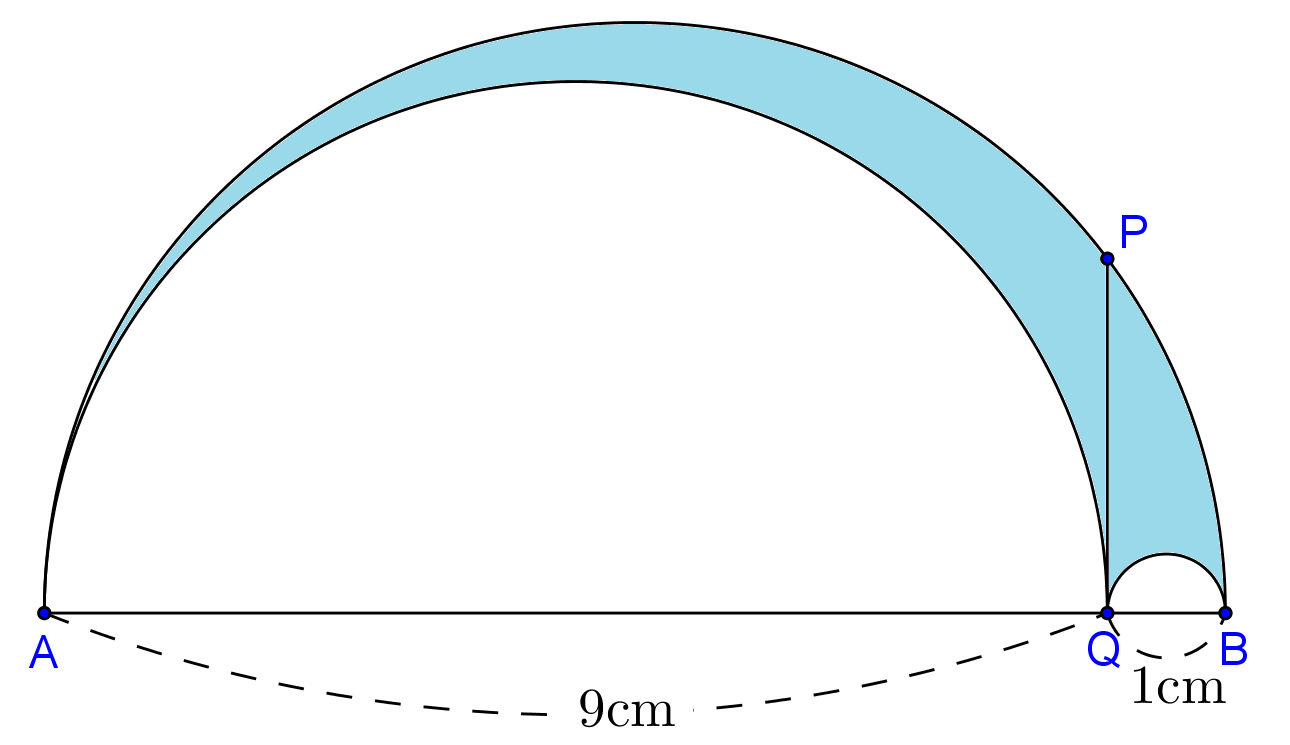
\includegraphics[width=0.6\textwidth]{1209a}
\end{figure}

%
\prob{1209a}\label{start}
\ov PQ를 지름으로 하는 원의 넓이를 구하여라.
\tabb{\frac74\pi}{\frac94\pi}{\frac{11}4\pi}{\frac{13}4\pi}{\frac{15}4\pi}

%
\prob{1209b}
색칠한 부분의 넓이를 구하여라.
\tabb{\frac74\pi}{\frac94\pi}{\frac{11}4\pi}{\frac{13}4\pi}{\frac{15}4\pi}

%
\prob{1209c}
\wh AB의 길이를 구하여라.
\tabb{3\pi}{4\pi}{5\pi}{6\pi}{7\pi}

%
\prob{1209d}\label{end}
\wh AQ+\wh BQ의 값을 구하여라.
\tabb{3\pi}{4\pi}{5\pi}{6\pi}{7\pi}

%
\prob{1209e}
\kswrapfig[Pos=r,Width=5cm]{1209e}{
오른쪽 그림에서 \ov AB는 반원 \(O\)의 지름이고, \(Q\)는 \ov AB 위의 점이다.
색칠한 부분의 넓이의 최댓값을 구하여라.
}
\tabb{\pi}{\frac94\pi}{4\pi}{\frac{25}4\pi}{9\pi}

%
\prob{1209f}
\kswrapfig[Pos=r,Width=5cm]{1209f}{
효원이는 다음과 같은 경로를 따라 \(A\)를 출발해 \(B\)를 거쳐 \(C\)에 도착한다.
걷는 속도는 \(2\pi\) m/s로 일정하고, \ov AC=40m일 때, 도착하는 데 걸리는 시간은 몇 초인가?
(단, 경로는 모두 반원이다.)
}
\tabb{8초}{10초}{12초}{14초}{16초}

\clearpage
아래 그림에서 \(\square ABCD\)는 한 변의 길이가 \(12\)인 정사각형이고 \(P\)는 \ov BD 위의 점이다.
\(\ov BP\), \ov PD를 각각 대각선으로 하는 정사각형 \(OBEP\), \(FPO'D\)를 만들고, \(O\), \(O'\)를 중심으로 하는 사분원 두 개를 만들었다.
다음 물음에 답하여라.
(문제 \ref{start'}--\ref{end'})
\begin{figure}[h!]
\centering
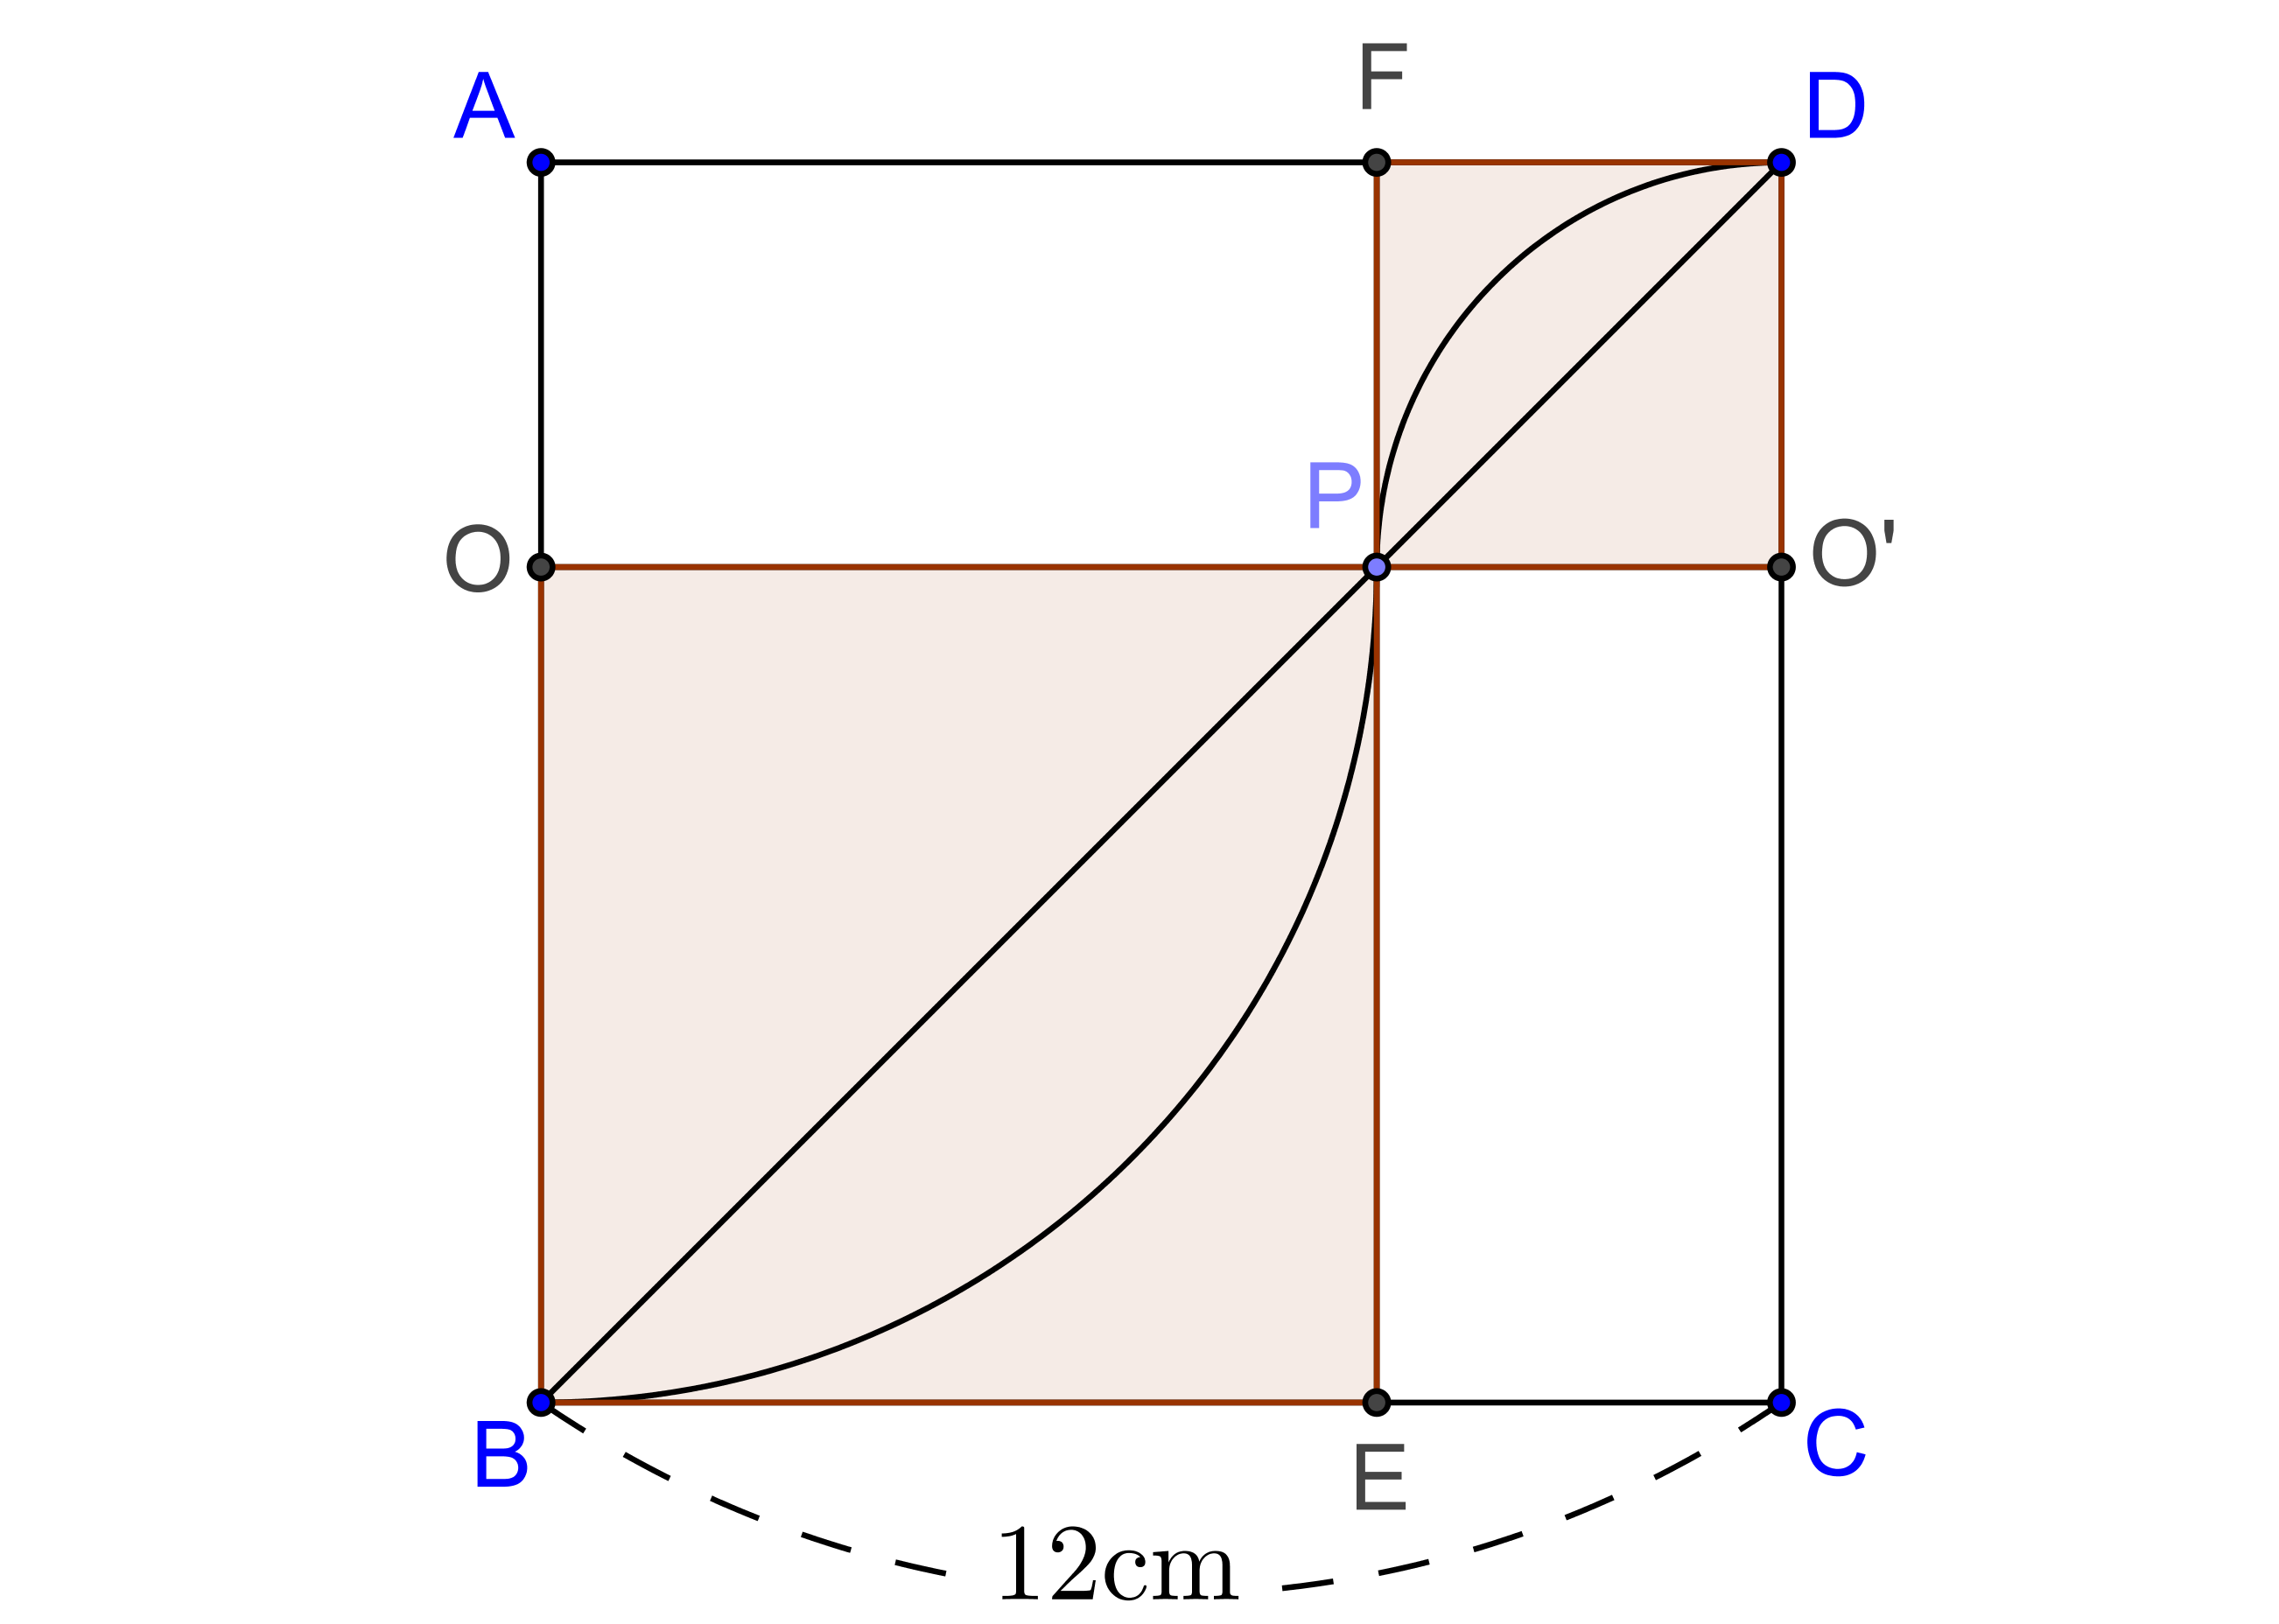
\includegraphics[width=0.6\textwidth]{1209g}
\end{figure}

%
\prob{1209f}\label{start'}
두 정사각형의 둘레의 길이의 합을 구하여라.
\tabb{45\text{cm}}{46\text{cm}}{47\text{cm}}{48\text{cm}}{49\text{cm}}

%
\prob{1209g}\label{end'}
두 사분원의 길이의 합 \(\left(\wh BP+\wh PD\right)\)을 구하여라.
\tabb{3\pi\text{cm}}{6\pi\text{cm}}{9\pi\text{cm}}{12\pi\text{cm}}{15\pi\text{cm}}

%%
%\prob{교과서a}
%\kswrapfig[Pos=r,Width=5cm]{text1}{
%오른쪽 그림에서 \ov AT는 원 \(O\)의 접선이고 \(\angle BAT=\angle CAB=36^\circ\)이다.
%\ov BP가 원 \(O\)의 지름일 때, \(\angle CAP\)의 크기를 구하여라.
%}
%\tabb{48^\circ}{54^\circ}{60^\circ}{66^\circ}{72^\circ}
%
%\clearpage
%%
%\prob{교과서b}
%\kswrapfig[Pos=r,Width=5cm]{text2}{
%\ov AT는 반지름의 길이가 \(2\)인 원 \(O\)의 접선이고 \(B\), \(C\)는 각각 \(\angle TAO\)의 삼등분선과 원 \(O\)의 교점이다.
%이때 \ov AC의 길이를 구하여라.
%}
%\tabb{\sqrt2}{\sqrt3}{2\sqrt2}{2\sqrt3}{3\sqrt2}
%
%%
%\prob{교과서c}
%\kswrapfig[Pos=r,Width=5cm]{text3}{
%오른쪽 그림에서 \ov AT는 원 \(O\)의 접선이고 \wh AB=\wh BC이다.
%\(\angle BAT=31^\circ\)일 때, \(\angle CAT\)의 크기를 구하여라.
%}
%\tabb{60^\circ}{62^\circ}{64^\circ}{66^\circ}{68^\circ}

%공통내접선
%공통외접선

\end{document}
